\section{Introduction}

\subsection{Chapter Outline}

In this chapter I analyse the evidence for key biological determinants of lymphatic filariasis (LF) transmission and use a model of transmission derived from branching process theory to demonstrate that a target threshold of $<$1\% microfilariae (mf) prevalence is not likely to be sufficient for transmission interruption in communities with a mid-to-high annual biting rate. I also show that the insufficient and inconsistent experimental evidence behind key biological determinants of disease, particularly the transmission rate from vector to human, leads to high uncertainty in confidence of elimination success. This highlights the need for further experimental studies to refine our understanding of LF thresholds. I then go on to describe how local biting rate or vector density could be used as a proxy for transmission intensity to adapt targets between settings. 

\subsection{Disclaimer}

This chapter is adapted from my first author article entitled \textit{Evaluating the evidence for lymphatic filariasis elimination}, published in Trends in Parasitology in November 2019 \cite{Davis2019} and also from a general audience article \textit{Is there a worm on that branch?} published in a Biology and Medicine Special Issue of Mathematics Today in October 2019 \cite{Davis2019_MathsToday}. I was the first author on both articles and the work contained is my own, conducted with consultation from and collaboration with the other authors. There is some additional content and detail that was not included in these publications, specifically expansion and integration of relevant supplementary materials.

\subsection{Background}

The year 2019 marks a number of important anniversaries: 75 years since D-Day, 50 years since both the Stonewall riots and the first moon landing and 30 years since the fall of the Berlin Wall. It also marks 40 years since the global eradication of small pox -- the first infectious disease to be driven extinct by modern medicine \cite{Breman1980}. Prior to eradication, small pox had existed for at least 3,000 years and, with up to a 30\% mortality rate, was considered one of the most feared human diseases in the world \cite{Hopkins2002}. Now, thanks to a global vaccination campaign, the virus is believed to only exist in two secure laboratories and there have been no reported cases since 1978.

The success of the small pox programme led to an increase in discussions about eradication of other diseases, such as polio, mumps and guinea worm. In 1993, The Carter Center, a not-for-profit organisation founded in 1982 by former U.S. President Jimmy Carter, published a report declaring these three diseases, along with three others, as potentially eradicable with existing tools \cite{Klepac2015}. Malaria eradication, previously abandoned after being unsuccessfully targeted in the 1950s and 60s, also made a return to the global health agenda in 2008 \cite{Feachem2008}. Whilst the only other disease to join small pox in the last 40 years has been rinderpest, a livestock disease eradicated in 1999 \cite{Morens2011}, there has been some significant progress made towards achieving elimination across number of these diseases. Notably, global efforts have brought cases of Guinea worm down from almost 100,000 in 1993 to only 30, from just two countries, in 2017 \cite{Molyneux2017}.

LF was one of the diseases earmarked for eradication in 1993 \cite{Klepac2015}. Colloquially known as elephantiasis, LF is a mosquito-transmitted worm infection that can cause lasting and debilitating disability if left untreated \cite{WHOLF}. Although reliable written records of the disease only date back to the 16th century, historians argue it has been around for a lot longer. Due to the distinctive nature of some disease symptoms, such as the severe swelling of limbs, there are ancient artifacts dating all the way back to Pharaoh Mentuhotep II's reign over Ancient Egypt around 2000 BC that potentially provide evidence of filariasis in the ancient world \cite{Kenawy2015} (see Figure \ref{fig:Pharoh}). 

\begin{figure}
    \centering
    
\includegraphics[height=15.3cm]{Project/Figures/LFElimination/Mentuhotep.jpg}
    \caption{A statue of Pharoah Mentuhotep  II (who reigned c. 2055--2004 BC). Swollen limbs, as are depicted here in the legs, are a characteristic symptom of lymphatic filariasis. Image credit: Statue of Nebhepetre Mentuhotep II in the Jubilee Garment MET DP302395.jpg by Pharos / Wikimedia Commons / CC0 1.0}
    \label{fig:Pharoh}
\end{figure}

Four-thousand years later, in AD 2000, infection was still widespread across tropical regions, with 120 million people estimated to be at risk \cite{Melrose2004}. Due to over 7 billion treatments being delivered through mass drug administrations (MDA, where large proportions of the population are treated at the same time, usually yearly), the number of infected people is thought to have lowered substantially since the millennium, with fourteen countries having been validated as reaching less than 1\% prevalence across their endemic regions \cite{WHOLF,WHOWER}. 

The question which now faces the Global Programme to Eliminate Lymphatic Filariasis (GPELF), is whether and where LF is likely to be eliminated once this low level of infection is achieved. The mathematical literature on infectious diseases has been crucial in informing the discussion on eliminating infections, and a number of challenges remain \cite{Klepac2015}. Here we address the particular challenges of modelling the elimination of a sexually reproducing parasite which is transmitted by a mosquito.

\subsection[Global situation]{Global situation and progress}

There are currently 886 million people across 52 countries worldwide at risk of LF \cite{WHO2019_FactSheet}. Infection is caused by a mosquito-transmitted filarial worm and, if left untreated, can lead to permanent and debilitating disability. GPELF set a target of elimination as a public health problem (EPHP, see Glossary) in 1997, leading to over 7.1 billion treatments delivered as part of mass drug administrations (MDA) since 2000 \cite{WHO2017_GPELF}. In 2011, the WHO published guidelines for halting treatment and verifying EPHP through the use of Transmission Assessment Surveys (TAS) to measure a target threshold \cite{WHO2017_Validation,WHO2017_Alternatives}. By October 2018, 14 countries had reached this target, and 554 million people worldwide no longer require mass treatments \cite{WHO2019_FactSheet}.

As indicated by the name of the TAS, it was hoped that reaching these targets would lead to elimination of transmission (EOT) in most areas. However, in Sri Lanka the TAS has been demonstrated as not sensitive enough to detect low-level persistence \cite{rao2014,rebollo2015} and pockets of transmission are still being found despite EPHP validation. The community is now revisiting the TAS methods, including the original target of 1\% microfilaria (mf) prevalence \cite{WHO2016}, particularly in the context of the new triple-drug regimen which is hoped to accelerate progress, but will require different post-treatment surveillance \cite{Irvine2017_Tripledrug}.

It is possible that achieving EPHP, according to the current definition, will lead to EOT in some settings \cite{DeJian2013,Won2018}, but the high levels of variability between localities and uncertainty in our knowledge of transmission makes it hard to predict where this will occur. This is exacerbated further by seasonal variation in environmental conditions, which has been shown to impact a number of helminth infections \cite{Davis2018,White2011}. Residual infection remaining after MDA cessation can lead to resurgence and reintroduction \cite{Xu2019,Singh2015}, with long-term persistence dependent on a range of factors \cite{Minetti2019}.

\section{Methods}

\subsection[Elimination theory]{Sexual reproduction in the host and elimination}

The sexual reproduction of filarial worms requires both male and female parasites to be present in an individual host for microfilariae production, so at a sufficiently low prevalence we would expect most infections to be non-transmissible due to low parasite load (i.e. a low probability of male and female adults in the same host). This is expected to result in fewer onward infections, and hence increasingly lower prevalence and intensity, until infection dies out. The threshold below which we expect this phenomenon to occur is called the breakpoint \cite{Anderson1992,Anderson2017}. As the focus of some NTD programs has shifted from control towards elimination, there have been a number of studies aiming to quantify these thresholds for a variety of helminth infections within the NTD umbrella \cite{Truscott2017,Irvine2018,Klepac2015,Hollingsworth2015}.

\begin{figure}
    \centering
    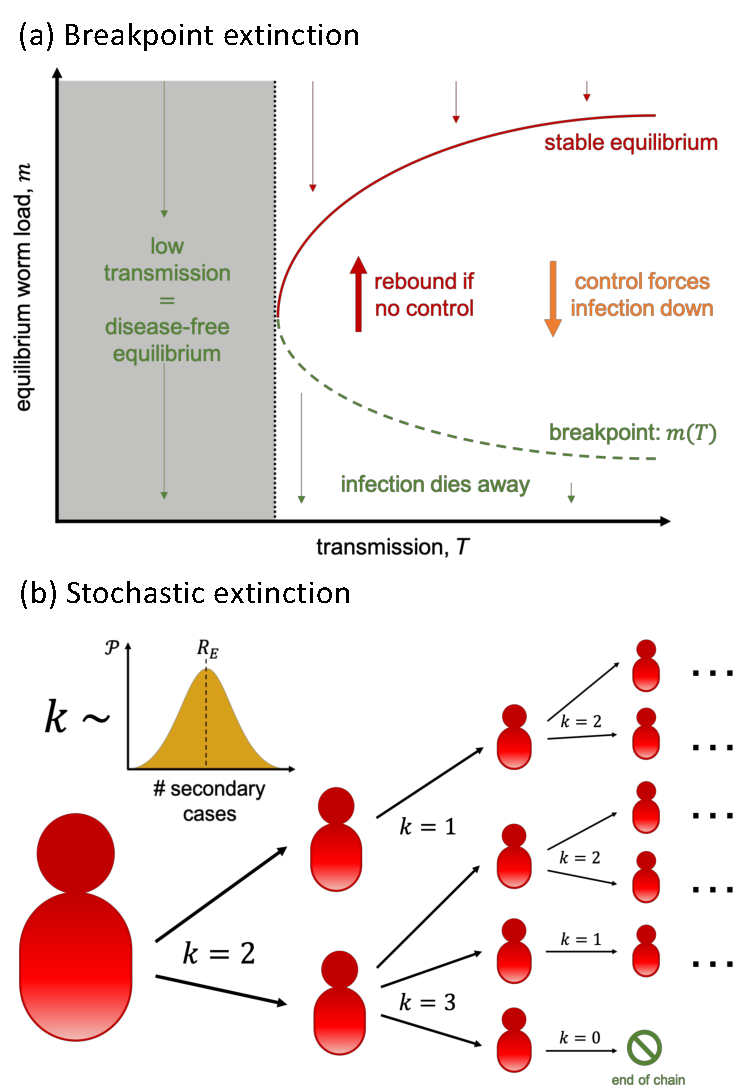
\includegraphics[height=15.3cm]{Project/Figures/LFElimination/Figure1.pdf}
    \caption{LF extinction theory. Schematics comparing the theory behind breakpoint extinction (a) and stochastic extinction (b) for LF. (a) For sufficiently low transmission intensities (i.e. low biting rates) disease levels will drop away to zero. Beyond the critical transmission level (black dotted line) there are three equilibria: high disease (stable, red), low disease (unstable “breakpoint”, green), disease-free (stable, black). Disease levels above the breakpoint will increase to the higher equilibrium, whereas disease levels below will decrease to zero. (b) Visual depiction of a transmission chain starting with one infectious individual. The number of secondary infections caused by each currently infectious individual are sampled from the secondary case distribution. This is used to simulate the onward chains of infection; extinction occurs when all chains die out (i.e. have no secondary cases). Stochastic variation can cause this to occur even above the theoretical breakpoint threshold.}
    \label{fig:Elim_1}
\end{figure}

This theory has certain consequences for control (Figure \ref{fig:Elim_1}a). If transmission is sufficiently low, then the infection is expected to die out. If there is a higher transmission rate, outcomes depend on the mean worm load in the population; if, usually through control strategies, the worm load is below the green dashed line (the breakpoint) then elimination is assured. Previous modelling studies that have assessed breakpoint thresholds have found values of much less than 1\% mf prevalence \cite{Singh2015,Michael2017,Michael2018,Gambhir2010}. It has been previously demonstrated that factors such as parasite aggregation and vector competence will further affect these thresholds \cite{irvine2015} and the majority of studies have focused on specific geographical areas, resulting in a wide range of suggested breakpoints across the literature.

Measuring breakpoints that are substantially lower than 1\% mf prevalence would require infeasible sample sizes and survey costs. In this review we don’t argue for a specific breakpoint, instead focusing on asserting that the experimental evidence is too uncertain to conclusively support a 1\% threshold and emphasizing the importance of spatial heterogeneity.

Whilst breakpoint theory is extremely useful, it is also possible for stochastic, or chance, extinction to occur before this break-point is reached, particularly when infection levels are low (Figure \ref{fig:Elim_1}b). The probability of elimination, given a particular prevalence (e.g. 1\%), can be calculated by considering the probability a chain of transmission will die out (this chain has similarities to a branching process \cite{Watson1875}). These types of branching-process-style methods have been used for soil-transmitted helminths \cite{Cornell2004_Stochastic,Cornell2004_Ultimate}, but have been adapted here to account for vector-borne transmission with an aggregated bite risk \cite{Fowler2016,Irvine2017_Mosquitobite}

Current guidelines mean EPHP is validated after passing TAS, but we have little experience in what this means for long-term transmission. Assuming for simplicity that TAS is able to measure a true mf prevalence of less than 1\%, this theory of stochastic extinction can be used to estimate how the future probability of EOT (zero infections) depends on a range of setting- and disease-specific variables. This process uses the distribution of the number of infectious secondary cases caused by one infectious individual, the mean of which is the effective reproductive number ($R_e$).

\begin{figure}
    \centering
    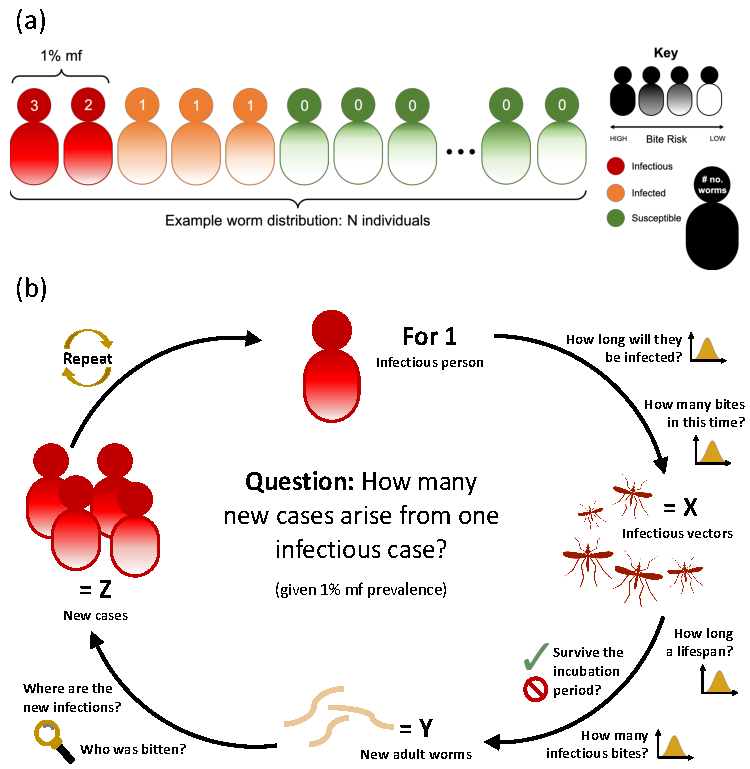
\includegraphics{Project/Figures/LFElimination/Figure2.pdf}
    \caption{Simulating transmission chain extinction. A schematic describing the simulation process for calculating the number of secondary cases produced by one infectious individual in a population with 1\% mf prevalence. (a) Allocate distribution of adult worms and bite risks across the population. Individuals with 1 worm are infected but not infectious, individuals with ≥2 worms are considered potentially infectious. (b) Generational calculation of number of new infectious cases caused by aan average infectious individual. One infectious individual infects $X$ vectors. The vectors that survive the incubation take infectious blood meals, resulting in $Y$ new adult worms. These worms are distributed across the population according to bite risk aggregation, resulting in $Z$ new infectious ($\geq$2 worms) individuals.}
    \label{fig:Elim_2}
\end{figure}

As a toy example, for a population of 1000 and 1\% mf prevalence, we consider a distribution of individual worm burdens (Figure \ref{fig:Elim_2}a). Infections with only one worm are non-transmissible. From one infectious person you then get the number of new cases, $Z$, caused during their infectious period (Figure \ref{fig:Elim_2}b). Since transmission represents a chance event, $Z$ is best represented by a distribution, and acts as a proxy for $R_e$. This distribution determines the probability of the transmission chain dying out, i.e. no further cases, at some point in the future. We use this to give a univariate demonstration of the present parameter uncertainty and how this might impact two epidemiological measures: the probability of elimination and the effective reproductive number.

\subsection[Branching processes]{Branching process extinction}
The most common branching process formulation is the Galton-Watson process \cite{Watson1875}, which we outline here before adapting for LF (Figure 3, right):

Let $X_n$ denote the number of infectious individuals in generation $n$ and for each infectious individual, $i$, let $Z_{n,i}$ be the number of new infectious cases directly caused by that individual. $Z_{n,i}$ iid random variables over $n\in{0,1,2...}$ and $i\in{1,...,X_n}$.

Assuming we start a chain of infection with one infectious individual, $X_0=1$, we then have the recurrence equation,
\begin{equation}
    X_{n+1} = \sum_{i=1}^{X_n}Z_{n,i}\,.
\end{equation}

The extinction probability of one chain of infection is the probability that $X_n=0$ for some $n>0$, or that $\lim_{n\rightarrow\infty}P[X_n=0]$.

Define $p_m$ ($m=0,1,2,...$) as the probability of an individual producing $m$ offspring and $d_m$ as the probability of extinction by the $m$th generation; $d_0=0$ as we start with one individual in generation $0$. Hence $d_m$ is an increasing, bounded sequence ($0=d_m\leq d_1\leq d_2\leq ... \leq 1$) and therefore converges to some limit, $d$, where $0\leq d\leq 1$ is the ultimate extinction probability.

\begin{eqnarray}
    d_1 &=& p_0 \\
    d_2 &=& p_0 + \sum_{j=1}p_j(d_1)^j\\
    &...&\\
    d_m &=& p_0 +  \sum_{j=1}p_j(d_{m-1})^j \,.
\end{eqnarray}

We can write this as,

\begin{equation}
    d_m = f(d_{m-1})
\end{equation}
where $f$ is the ordinary generating function:
\begin{equation}
   f(d) = p_0 +  \sum_{j=1}p_jd^j \,.
\end{equation}

Since $d_m\rightarrow d$, we can find the probability of ultimate extinction by solving $d=h(d)$. 

We want to show that $d$ is the smallest non-negative root of this equation. Take $b>0$ also a root with $b\neq d$ and $b=f(b)$, then we have that $d_1=f(0)\leq f(b)=b$, hence $d_1\leq b$. Assume $d_k\leq b$ for some $k$, then

\begin{equation}
    d_{k+1} = f(d_k) \leq f(b) = b \,,
\end{equation}

since $f$ is an increasing function. Hence, by induction $d$ is the smallest non-negative root. The function, $f$, is also convex and hence has at most two real roots. Since one is always a root, $f(1)=\sum_{j=0}p_j=1$, then the probability of ultimate extinction is only less than one if the second root both exists and lies between zero and one. 

By considering the gradient of $f$ at one, $f'(1) = \sum_{j=1}jp_j$, we can determine the location of the other root -- namely there is only a second root in $[0,1]$ if $f'(1)>1$. Notably this gradient, $f'(1)$, is equal to the average number of secondary cases caused by a single infectious individual, often called the basic reproduction number to describe early outbreak dynamics. Since we are considering a situation where there is a background population prevalence that has been artificially lowered to 1\%, we call this the effective reproduction number, $R_e$.

In our model (further details below), we want to take account of the heterogeneous worm distribution across hosts, as it is a key feature of the system. Therefore, it is not possible to directly calculate either the effective reproduction number or the probability of extinction, but both can be calculated numerically by considering the outcome distributions of stochastic simulations. In particular, by calculating the proportion of simulated individual infections that result in each number of onward infections, we can generate a discrete numerical approximation of our secondary case offspring probability distribution. 

From this, we can iterate through each generation to find the probability that extinction has occurred. This probability converges over time and, if sufficient generations are considered, can be used as an approximation of the ultimate extinction probability, $d$.

\subsection[LF model]{Lymphatic filariasis model}
In order to estimate the extinction probability for LF, we simulate a population of 1000 individuals, with variable infection risk, of whom 1\% are productively infected (producing transmissible offspring, mf), a proportion are unproductively infected and the remainder are uninfected. We assume the dominant vector is \textit{Anopheles gambiae}. 

We then calculate for a randomly infected individual, the number of onward productive infections they produce according a model of the life-cycle. An infection lasts for a randomly selected period of time (exponential, mean $1/r$, the estimated fecund life span, 6 years). This individual has a risk of being bitten relative to the rest of the population (Gamma, mean=1), which, depending on the annual bite rate (ABR), or the expected number of bites per year, generates the expected number of bites in during their infectious period. For each bite, there is a probability, $c$, that the mosquito becomes infected. We assume each new infection occurs in a new mosquito, which gives an upper bound of the total number of infected mosquitoes for this individual.

Each mosquito then has exponentially distributed life expectancy (mean$=1/g$, 6.9 days \cite{Killeen2000,Subramanian1998}) and has to survive an incubation period (also Exponential, mean$=\nu$, 8.5 days \cite{erickson2009}). From this we can derive the probability a vector survives to infectiousness and, using a binomial distribution, calculate the total number of infected vectors, $V$, which survive the incubation period. The number of infectious bites caused by these vectors is then Poisson distributed at a daily rate, $f$=0.335 \cite{Subramanian1998}, per vector and of these bites only a small proportion, $b\ll1$ \cite{Hairston1968,Jones2014}, will successfully lead to a productive infection. The efficacy of transmission from vector to host is so low due to the route the larvae must take to establish; rather than being injected into the bloodstream during the bite, the larvae must instead independently fall onto the skin and find the hole left by the mosquito after feeding.

This describes the number of new adult worms $Y$, that are established in humans resulting from the entire duration of this one individual's infection (one distinct outcome per iteration, creating a distribution). From the total number of new adult worms, $Y$, we can derive the effect on prevalence by sampling $Y$ individuals, with replacement, according to bite risk. Each time an individual is sampled they gain 1 adult worm. We then compare new worm burdens with previous worm burdens -- how many new infectious ($\geq 2$ worms) cases are there that were previously not infectious ($\leq 1$ worm)? This gives our number of secondary infections, $Z$.

Then the mean number of new infectious humans is $R_e$, which here relates to the full-cycle reproduction number focusing on human infections only. If $R_e<1$ then eventual extinction will occur -- implying that prevalence is already below the theoretical breakpoint of the system. However, if $R_e>1$ then extinction is not guaranteed but may still occur. We need to consider the offspring distribution of the transmission chain, $p_j$ probability of having $j$ secondary cases, which can be approximated by the scaled frequency of secondary infectious case counts, in order to calculate the probability of extinction.

\section[Life-cycle variables]{Empirical evidence for life-cycle variables}

We now review evidence for key parameters in the life-cycle which drive transmission (Figure \ref{fig:Elim_3}). As previously mentioned, a number of these variables, such as the annual biting rate (ABR), are likely to introduce large differences due to the high spatial variability. Others, such as the probability an infectious mosquito bite results in a viable human infection, have the potential to be more consistent across settings, but currently lack in experimental evidence. Table \ref{tab:Elim} at the end of this section outlines the range of values for biological variables found in the literature. 

\begin{figure}
    \centering
    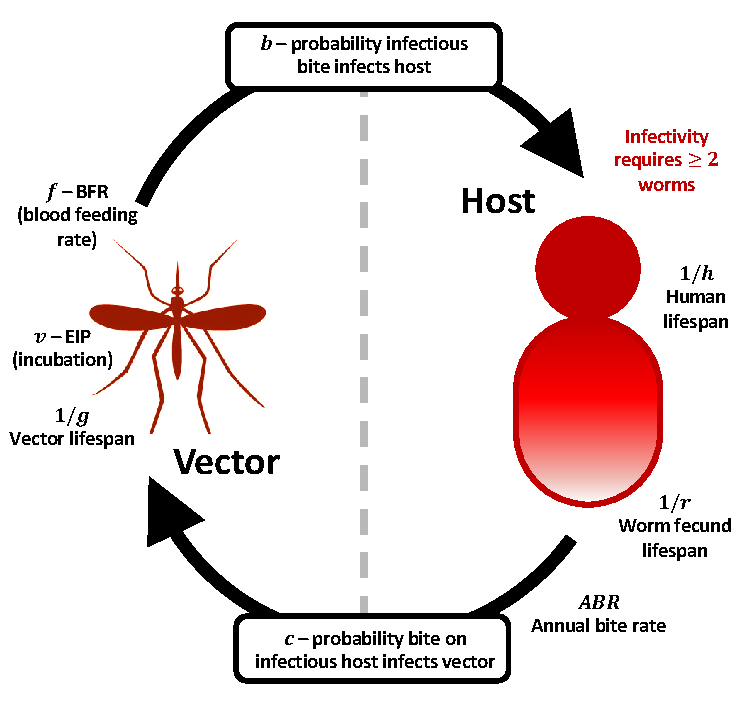
\includegraphics{Project/Figures/LFElimination/Figure3.pdf}
    \caption{LF life-cycle. Life-cycle schematic demonstrating key biological variables that could affect prediction of elimination success. Duration of infection is determined by human and fecund worm lifespans. Infection from host to vector depends on the annual biting rate (ABR) and the probability a bite on an infectious host infects a vector. The number of vectors that survive to infectivity depends on incubation (EIP) and vector lifespan. Transmission from vector to host is then determined by the blood feeding rate and the probability an infectious bite results in a viable adult infection, as well as the requirement for $\geq$2 worms for infectivity.}
    \label{fig:Elim_3}
\end{figure}

A detailed literature review turns up widely varying estimates of ABR, partially due to geographical variation. These values, from countries with history of LF endemicity, range from 3 \cite{Killeen2000} to 611 \cite{Michael2016} bites per person per day. A number of these are based on human landing catches \cite{Killeen2000,Michael2016,Braack2015}, with the majority relying on studies from the 1960s and 70s \cite{Michael2016}, whilst some are derived from models \cite{Stolk2005}. Despite a wealth of historic studies, supported by the malaria literature (which covers many of the same vector species including \textit{Anopheles gambiae}), human landing catches are often considered unethical and give highly variable results. Relying on historic estimates can also disregard changes in socio-economic conditions resulting in decreased vector-human contact.

Current estimates in the literature of the basic reproductive number without control, $R_0$, range from 0-2.5 \cite{Stone2014}, depending on the vector-host ratio (an alternative metric to ABR). Although setting-specific values of $R_0$ for other diseases can often be calculated from infection data, the global landscape of public health history for LF means that we have very little contemporary baseline (pre-control) data with which to do this. As an alternative, we can consider the previously mentioned estimation of $R_e$.

Another important, but largely uncertain, factor is the degree of parasite aggregation, measured inversely by the negative binomial $k$. For LF, adult worm aggregation is considered to be driven by heterogeneous transmission, caused by host variation in bite risk \cite{Irvine2018}. Initial estimates for $k$ were based on mf data ($k$ = 0.08, 0.3 \cite{irvine2015,Irvine2017_Mosquitobite}). However, a recent study in Papua New Guinea used bite and mf data to demonstrate that the $k$ for bite risk is an order of magnitude larger than that for mf aggregation, giving a refined estimate of 0.73 (s.d. 0.035), with site-specific estimates ranging from 0.3--1.3 [15, 26]. We will now separate transmission into two parts: humans to mosquitoes, and mosquitoes to humans. When considering the former the key variables are duration of infection, which depends on fecund worm lifespan, and the probability that a vector biting an infected host will become infectious. 

Often worm lifespan is stated as being 6-8 \cite{WHO2019_FactSheet} or 5-10 years \cite{Norman2000_epifil,Stolk2006}, but reference trails rarely reveal empirical evidence. There are studies that corroborate similar ranges, such as 2.1-5.4 \cite{Vanamail1996} or 9.1-11.8 \cite{Subramanian2004} years, but there are also estimates in the literature of up to 40 years \cite{Carme1979}.

Infectivity to mosquitoes depends on mf intensity, leading to wide ranges of 15-60\% of vectors becoming infected from a single mf positive bite \cite{Subramanian1998,gambhir2008}.

Infection from vector to human is governed by the number of infectious bloodmeals one mosquito will take – calculated from vector survival and competence, extrinsic incubation period (EIR) and blood feeding rate (BFR) – and the probability one infectious bite will result in a viable infection. There are reasonable estimates for vector survival and BFR from the malaria literature \cite{Killeen2000,Gary2001} and for LF incubation \cite{erickson2009}, although these do not typically account for the impact of infection on survival \cite{Subramanian1998}. 

One key parameter of infection, the probability an infectious bite results in a mature human infection, is largely unknown. Estimates range from 10-5 to 10-3 \cite{Hairston1968,Jones2014} and are usually broken down into three steps: the L3 leaving the vector, entering the host and developing to fecundity. The first is relatively straightforward to measure \cite{deMeillon1997}, although poses ethical issues, and the second can be estimated using mouse models \cite{Ho1967,Ewert1967}. The third is harder; best estimates are calculated by using \textit{Brugia malayi} studies to derive a daily death rate and then applying this across the longer \textit{Wucheria bancrofti} developmental period \cite{Norman2000_epifil,Addiss2000}. Although \textit{Brugia malayi} is also a cause of LF in humans, the parasite is of a separate species to \textit{Wucheria spp.} and hence is not necessarily comparable in this way. 

\begin{sidewaystable}[p]
    \centering
    \begin{tabular}{|l|p{70mm}|p{95mm}|1|}
    \hline
    \multicolumn{1}{|l|}{\bf Item} & \multicolumn{1}{|l|}{\bf Biological meaning} &
\multicolumn{1}{|l|}{\bf Range of estimates} &
\multicolumn{1}{|l|}{\bf Mid-point} \\ \hline
        $\psi_1$ & Prop L3 leave vector per bite & 0.437(\textbf{0.363 -- 0.511})\cite{deMeillon1997}, 0.414 \cite{deMeillon1997} & 0.437  \\
        $psi_2$ & Prop L3 enter host & 0.223 \cite{Norman2000_epifil,Ewert1967} & 0.223 \\
        $w$ & Developmental period in host & \textbf{6 months 9 days -- 12 months 14 days} \cite{Addiss2000}, 8 months 4 days \cite{Hairston1968} & \\
        $s_2$ & Prop L3 develop to adulthood & (\textbf{0.036 -- 5.68})$\times 10^{-3}$ \cite{Hairston1968,gambhir2008,erickson2009,Jones2014} & 0.437$\times 10^{-3}$ \\
        $b$ & Probability infectious bite infects human & $=\psi_1\psi_2 s_2$ = (\textbf{0.15 -- 9.29})$\times 10^{-4}$, 1/47$\times 10^{-3}$ \cite{Hairston1968,Jones2014} & 1.43$\times 10^{-4}$ \\
        $ABR$ & Annual biting rate & \textbf{1129} \cite{Killeen2000}, 1500 \cite{Michael2016}, 22320 \cite{Braack2015}, 24090 \cite{Killeen2000}, 26400 \cite{Stolk2005}, 41975 \cite{Braack2015}, \textbf{69120} \cite{Stolk2005}, 223000 \cite{Michael2016} & 24090 \\
        $1/g$ & Vector life span (days) & \textbf{5.4 -- 9.5} \cite{Killeen2000,Subramanian1998} & 6.86 \\
        $1/r$ & Worm fecund life span (years) & \textbf{2.1} \cite{Vanamail1996}, 5.4 \cite{Vanamail1996}, 9.1 \cite{Subramanian2004}, \textbf{11.8} \cite{Subramanian2004}, 40 \cite{Carme1979} & 6 \\
        $c$ & Probability infectious bite infects vector & 0.37 \cite{gambhir2008} (\textbf{0.15--0.6}) \cite{Subramanian1998} & 0.37 \\
        $v$ & Extrinsic incubation period (days) & \textbf{7 -- 10} \cite{erickson2009} & 8.5 \\
        $f$ & Daily vector blood feeding rate & \textbf{0.26 -- 0.41} \cite{Subramanian1998} & 0.335 \\
        $k$ & Parasite aggregation & \textbf{0.08 -- 1} [various] & 0.5 \\
        \hline
    \end{tabular}
    \caption{Values for biological variables found in the literature, which were used in the calculation of results shown in Figure \ref{fig:Elim_4}. Values taken as maximum and minimum estimates for analysis are indicated in bold and mid-value estimates are listed separately. Mid-value estimates that are not also listed in the “Range of estimates” column are chosen to represent a mid-ground, usually an average of the maximum and minimum values.}
    \label{tab:Elim}
\end{sidewaystable}

\section[Results]{Results}

\begin{figure}
    \centering
    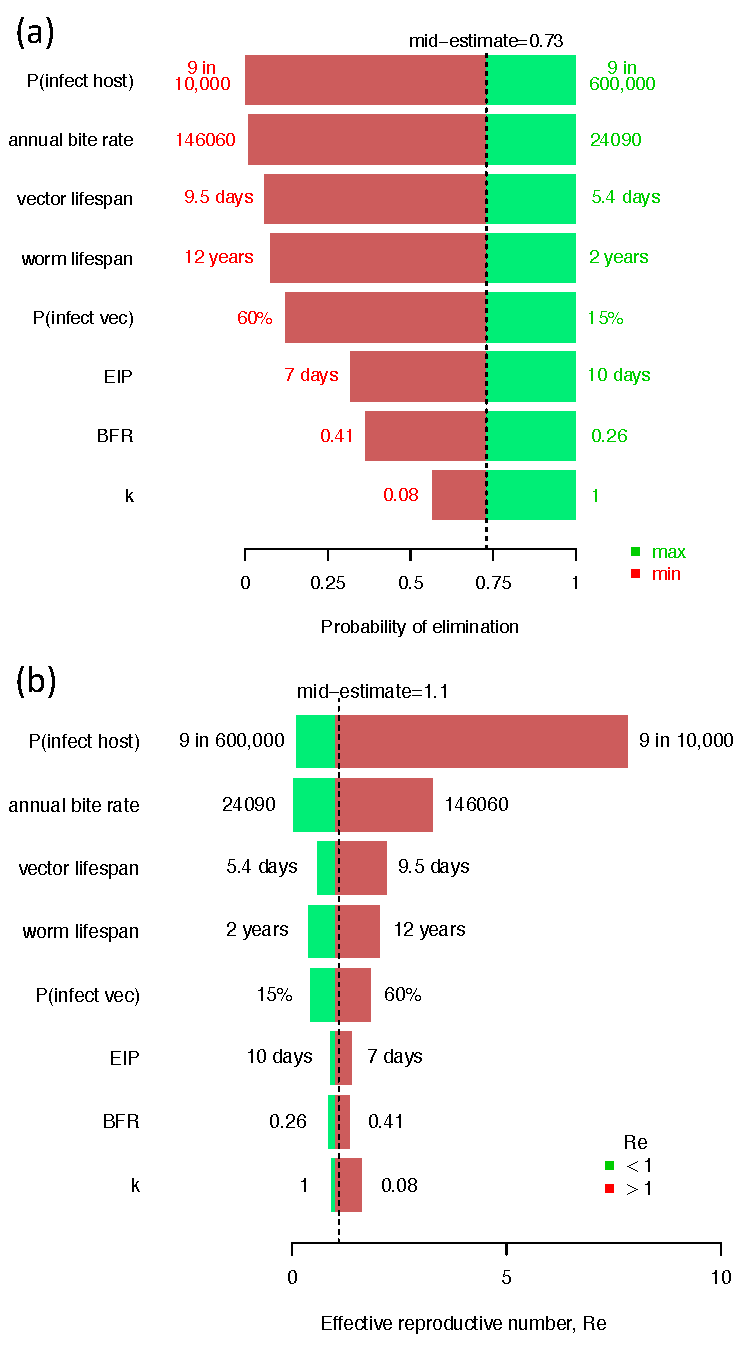
\includegraphics[height=16cm]{Project/Figures/LFElimination/Figure4.pdf}
    \caption{Predicting elimination probabilities. Illustration of the potential impact of high uncertainty in variables by considering their univariate impact on the probability of elimination (a) and the effective reproductive number (b) for the key biological variables of the LF transmission cycle. Assuming an mf prevalence of 1\% and a human population size of 1000. References for ranges of variables considered can be found in Table \ref{tab:Elim}. Note that this univariate analysis should be interpreted carefully as variables are likely to be correlated in ways which we cannot yet account for. For example, the mid-estimates here have been chosen to represent a mid-ground of ranges found in the literature and are not necessarily representative of the true values or ranges that may exist across real-world settings.}
    \label{fig:Elim_4}
\end{figure}

If we include these parameters in the simple framework described above, we can see how the uncertainty affects our estimates of key epidemiological measures (Figure \ref{fig:Elim_4}). The mid-points of elimination probability (0.73) and $R_e$ (1.1) are not intended to be true estimates, rather they represent a mid-ground of the parameter ranges found in the literature and a basis for comparison. 

The variable which generates the most univariate uncertainty is the probability an infectious mosquito bite will infect a human, $b$, due to the wide range of possible values. Variation in elimination probability due to ABR, which is correlated with the basic reproductive number ($R_0$), is also very high. This is due to both measurement inaccuracy and spatiotemporal variability. Parameters that are known to be key drivers in the probability of elimination, worm fecund lifespan and the degree of adult worm aggregation \cite{irvine2015,Truscott2017,Anderson2014}, potentially induce lower uncertainty here due to considering narrower plausible intervals.

In addition to the probability of elimination, we also consider the effective reproductive number, $R_e$. It is important to note that for helminth infections, metrics often refer to the number of adult filarial worms arising from one adult filarial worm, rather than considering human infections. However, the theory is similar enough to allow heuristic comparison. Our mid-estimate for $R_e$ is chosen to be close to 1, representative of the low-level transmission observed in some post-MDA settings, but varying the probability an infectious mosquito bite will lead to a patent infection ($b$) can lead to an order of magnitude difference. In fact, it is possible to push the estimate of $R_e$ across the critical threshold ($R_e=1$) between extinction and endemicity by adjusting any variable within the ranges found in the literature. This reinforces the importance of using reliable variable estimates when making predictions, particularly in elimination settings where infection data are sparse. 

We can characterise the probability of extinction from achievement of 1\% mf prevalence in relation to transmission intensity (Figure \ref{fig:Elim_5}, orange curve). When the annual biting rate (ABR) is low, then infection is highly likely to fade out, but this probability declines as the biting rate increases. This emphasises the importance of local context in determining the extinction probability from this endpoint. We additionally simulated the curve for a halving of the endpoint - a prevalence of 0.5\%. This, of course, increases the probability of extinction, but would require much larger sample sizes to evaluate. 

\begin{figure}
    \centering
    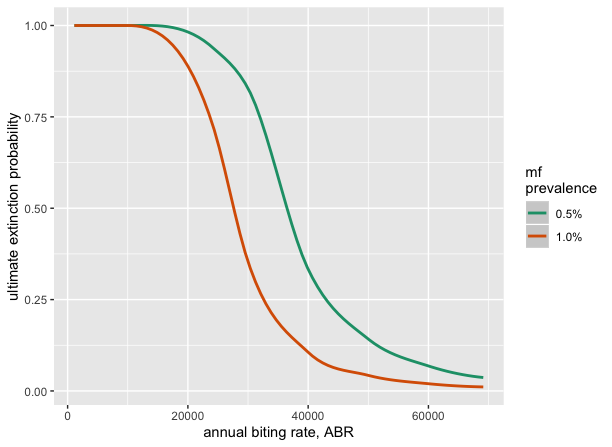
\includegraphics[height=10cm]{Project/Figures/LFElimination/Figure5.png}
    \caption{The probability that transmission will become extinct for different annual biting rates (ABR) and different starting prevalence (green 0.5\%, orange 1\%).  At low biting rates, the infection is highly likely to fade out, but for high biting rates it is unlikely.}
    \label{fig:Elim_5}
\end{figure}

\section{Recommendations}

Due to the demonstrated uncertainty that knowledge gaps, particularly in the establishment of a patent infection, can cause in estimating elimination thresholds it would be prudent to refine the evidence for these variables. Here we discuss a few options for future studies and analyses that we believe could strengthen the knowledge base.

The probability that an infectious bite leads to an infectious host cannot be measured experimentally in humans, however we can improve current estimates with anecdotal and observational studies. Longitudinal studies can provide evidence of the time to antigen positivity and the time to mf positivity in children, or in adults that have moved from non-endemic to endemic regions. One existing study, looking at acquisition in travellers, surmises that the majority of cases are in individuals who spent in excess of six months in an endemic region [49], whereas another cites a number of travellers contracting infection with only one month of exposure \cite{Jones2014}. Entomological studies routinely estimate ABR through human landing catch data, and individual exposure can be quantified based on net usage and vector biting habits \cite{Reimer2013_insecticidal,Thomsen2017}.

The range of ABRs discussed are very broad estimates, covering a wide range of settings, but this can be a difficult variable to measure consistently. It may be possible to obtain greater certainty in $R_e$ without accurate ABR measures for each location. For example, estimates of low, medium or high vector densities would still improve our predictions and these categories of exposure, which act as a proxy for $R_0$ classification, could be informed by a combination of trap densities and vector control coverage. Spatial heterogeneity can also occur within implementation units, posing problems for any categorisation process, so it is important that treatment targets are determined by the maximum transmission measure for a region. 

We have used basic analyses to highlight that the existing experimental evidence does not afford a high degree of certainty at the current 1\% mf prevalence elimination threshold. This is mainly because of uncertainties in variables which could be either experimentally or analytically refined, but also due to spatiotemporal variation in vector densities and biting rates \cite{Michael2016}. That varying the value of one input variable within sensible ranges found in the literature can make such an impact on predictions, demonstrates the difficulties posed by targeting EOT when we know local heterogeneities and variability are difficult to measure. Observations of ongoing transmission in parts of validated countries offer empirical support to our concerns with the EPHP target, prompting some important outstanding policy questions. This highlights the need for both refinement of the experimental evidence based and care when selecting model parameters from the literature.

Recent empirical evidence suggests the current survey does not capture ongoing transmission. By altering the survey design, through different diagnostics, measuring mosquitoes or sampling on a more detailed spatial scale, it is possible that areas of high transmission rates could be picked up earlier. In order to support efforts to eliminate lymphatic filariasis we would recommend a multi-pronged approach: improving the experimental evidence base of measurable quantities; detailed analysis of existing infection data to improve our understanding of the infection risk associated with an infectious bite; and development of a discrete system to classify vector density, as a proxy for transmission intensity, to allow comparison of different regions. The optimisation of elimination program strategies and surveillance will require continual revisiting of predictions as we gather more epidemiological data through existing surveys and monitoring infrastructures, as well as expanded epidemiological and surveillance studies at low prevalence. 

As more countries cease interventions and move to post-validation surveillance it is increasingly obvious that transmission breakpoints are unlikely to be one-size-fits-all, hence more flexible thresholds are necessary. The GPELF currently has only one surveillance strategy for all locations with the same mosquito and worm species. Fully tailoring strategies to local epidemiology would improve utility, but the cost of evaluating the local epidemiology is likely to far exceed the cost of the existing surveys. Therefore, it is likely that an adaptive survey design would be more practically useful. It is vital that we ensure this process is well-informed, as prematurely halting control or surveillance programs could pose a serious threat to global targets, but also because we believe that it may be possible to exploit this geographical variation to maximise the probability of elimination.


\section[Outstanding questions]{Outstanding questions and further work}

There remain a number of key outstanding questions surrounding the issue of LF elimination. In particular, the expected time frame of disease extinction is of increasing interest to public health initiatives and donors, who want to see return on their investments of time and money. Further analysis using the theory of branching processes could allow us to consider the likely timelines to extinction or elimination for scenarios that have $R_e<1$. However, as we know from well-established analysis of the deterministic model, the epidemic growth rate for a helminth with a lifespan of the order of a decade is extremely slow \cite{Anderson1992}. This means that for a number of the branches/simulations, infection can oscillate around low levels for many years before either re-emerging or fading out. This is a challenge that will require investment in long-term surveillance.

In addition, despite general agreement on the existence of a break-point, there is currently no clear consensus on where this threshold lies and how it might vary between different settings. Our results show that factors such as ABR could have a substantial impact on extinction probability, making it unlikely that there is a single threshold that will work reliably. However, this raises the question of how adaptable targets should be and how public health policy makers can best balance costs with setting appropriate and relevant targets. Indeed, if in some locations the break-point is lower than can feasibly be measured through current surveillance strategies, then what should the next steps be? It is currently unclear.

The impact of ABR on extinction probability for different thresholds is also interesting from the perspective of vector control initiatives. Decreasing the ABR in an area will increase the probability of disease extinction at a particular mf prevalence threshold, but we could also think about this in terms of how it affects the breakpoint; a lower ABR will give the same extinction probability for a higher mf prevalence. Looking back at Figure \ref{fig:Elim_1}, ABR can be considered a proxy for transmission intensity and decreasing transmission results in a higher breakpoint. If transmission is low enough then disease cannot be maintained at any prevalence and we would expect reversion to the disease-free equilibrium. In the next chapter I use a vector-based model to investigate the potential effect of vector control on transmission measures.

Another key unknown is how much of the uncertainty described here is due to lack of rigorous biological evidence and how much represents natural stochastic variation within nature. To quantify this will require well-formulated experimental studies and innovative ways of measuring key biological determinants of transmission. 

\section{Concluding remarks}

The elimination of an infectious disease requires a number of pieces of the puzzle to work together. Biological plausibility, usually due to the availability of a particular tool, such as a vaccine, or drugs donated for MDA, together with political will and funding at all levels, from global policy to community-level acceptability, are essential parts of the puzzle. Mathematical modelling can inform our understanding of the biological plausibility, identifying important drivers of success and informing the design of not only interventions, but how targets are set, measured and evaluated. 

In the case of LF, hopes for elimination in the coming decades are high. The slow epidemic growth rate, the lack of amplification in the mosquito (a mosquito can only transmit as many worms as they ingest, usually fewer), the low probability of infection of a host and the hope that global development will improve the living conditions of those exposed to these diseases, mean that there are many reasons to expect that elimination is likely to occur in many affected areas once infection is brought low, as this analysis suggests. The transmission chain model presented here, whilst mathematically relatively straightforward, provides a practical basis for informing policy discussions in this area. In particular it shows that there are likely to be many areas where additional interventions and surveys may be needed.

\subsection{Chapter summary}

In this chapter I described the history of disease elimination and introduced the disease of focus: lymphatic filariasis. I discussed the biology of transmission, namely the dependence of infectivity on parasite sexual reproduction in the host and how this creates a break-point prevalence where transmission is no longer viable. I also introduced the idea of stochastic elimination prior to reaching this break-point and used branching process theory to describe a model of transmission that could predict elimination probability for a specified set of biological parameters. I presented the results of a detailed literature review that determined possible ranges for these biological parameters and demonstrated how the wide variety of values found could have dramatic effects on model results. I then analysed my model output, showing the wide window of elimination probabilities and effective reproductive numbers that came from these parameter ranges, and discussed how the break-point might vary between settings -- specifically with regards to annual biting rate. I concluded by discussing the implications of these findings and outlining what further work could be done.